\section{Clustering}

Première observation pour le clustering: Plusieurs des méthodes proposées par Weka reposent sur d'autres métodes.

Ainsi, FilteredClusterer et MakeDensityBasedClusterer demandent de choisir une méthode de clustering parmis celles mises à disposition par Weka.
Petite particularité de Weka: Celui-ci n'empêche pas d'indiquer à (par exemple) FilteredClusterer d'utiliser FilteredClusterer pour fonctionner, permettant ainsi de "chaîner" indéfiniement ceux deux méthodes de clustering.
Après plusieurs tests, ceci ne change rien aux valeurs de résultats (mais augmente le temps de génération de ceux-ci).

Deuxième observation: D'autres méthodes permettent de définir un algorithme de calcul de distance parmi ceux proposés par Weka.

Ainsi, HierarchicalClusterer et SimpleKMeans sont tous les deux configurable à ce niveau.

Dans notre cas nous avons choisi de détailler les résultats de la méthode FarthestFirst car sa simplicité permet d'en combiner l'usage avec les cluster FilteredClusterer et MakeDensityBasedClusterer et bien comprendre son fonctionnement facilite ainsi la compréhension d'autres méthodes que nous pourrions combiner avec lors de cas extra-académiques.

La méthode FarthestFirst est dite de clustering non-hiérarchique (ou Flat Clustering) car elle ne crée par d'arbre, et donc pas de descendance / hiérarchie entre les cluster qu'elle génère.
Deux paramètre numériques sont définissables:
\begin{itemize}
	\item{Le nombre de cluster à générer}
	\item{La graine à utiliser pour tirer aléatoirement des exemples}
\end{itemize}

Contrairement à d'autres méthodes essayées et évaluées, FarthestFirst ne tire par une graine aléatoirement quand elle est définie à zéro.
Il est donc du devoir de l'utilisateur de Weka d'être attentif à cette particularité s'il souhaite lancer plusieurs générations affin de déterminer les meilleurs clusters possible.

Les options ne permettent pas de définir un nombre maximum d'itérations, on peut donc en déduire que la méthode évaluée repose sur la convergeance des données dans les clusters pour déterminer quand s'arrêter.

Pour nos tests nous avons essayez avec les nombres de clusters suivants:
\begin{itemize}
	\item{2: C'est le nombre minimum de clusters assignable et celà permet de voir quels données sont dissociées}
	\item{8: C'est le nombre de type de données différentes que nous traitons dans cet exercice}
\end{itemize}

\subsection{2 clusters}

Les listes déroulantes du haut de l'interface permettent de définir les éléments à afficher sur l'axe des X et ceux à afficher sur l'axe des Y pour la visualisation.
Si les types de données sont discrêtes, un paramêtre (jitter) permet de visualiser plus facilement l'étendue des répartitions en ajoutant une forme de bruit en X et en Y aux graphes.
Dans les exemples si dessous, les graphes sont fait avec le revenu annuel en abssisse et la possession ou non de maison en ordonnée.
En rouge et en bleu on voit les deux clusters déterminés par le run, dont le résultat est également ci-joint.

\begin{figure}[H]
\centering
\begin{lstlisting}
=== Run information ===

Scheme:       weka.clusterers.FarthestFirst -N 2 -S 0
Relation:     QueryResult-weka.filters.unsupervised.attribute.Remove-R2-7,9,11,14,16,18,21-25-weka.filters.unsupervised.attribute.Remove-R1
Instances:    18484
Attributes:   8
              MaritalStatus
              Gender
              YearlyIncome
              TotalChildren
              EnglishEducation
              EnglishOccupation
              HouseOwnerFlag
              NumberCarsOwned
Test mode:    evaluate on training data


=== Clustering model (full training set) ===


FarthestFirst
==============

Cluster centroids:

Cluster 0
     M M 60000.0 2.0 Partial College Professional 1 1.0
Cluster 1
     S F 170000.0 4.0 Bachelors Management 0 4.0



Time taken to build model (full training data) : 0.07 seconds

=== Model and evaluation on training set ===

Clustered Instances

0      14166 ( 77%)
1       4318 ( 23%)
\end{lstlisting}
\caption{Output de l'éxécution avec 2 clusters}
\end{figure}

\begin{figure}[H]
    \centering
    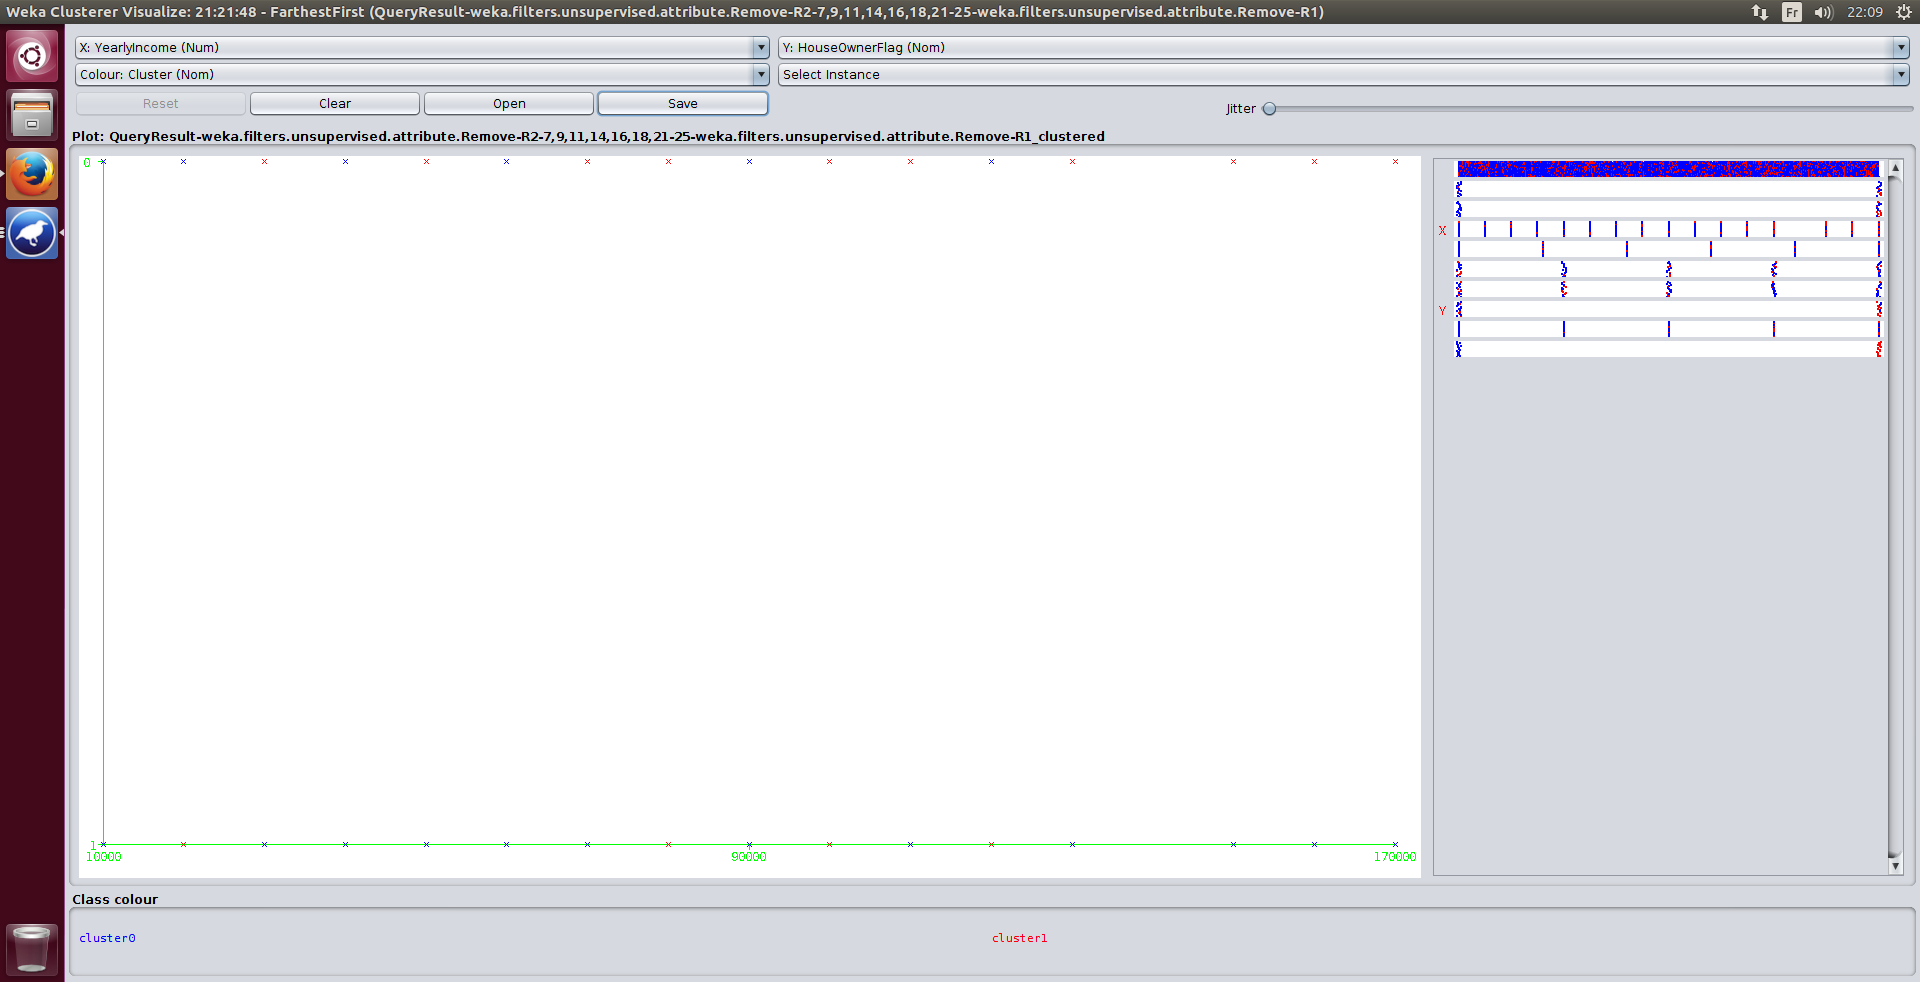
\includegraphics[width=1\linewidth, fbox]{img/clusterSansJitter2.png}
    \caption{Clustering sans jitter et avec deux clusters}
    \label{sansJitter2}
\end{figure}

\begin{figure}[H]
    \centering
    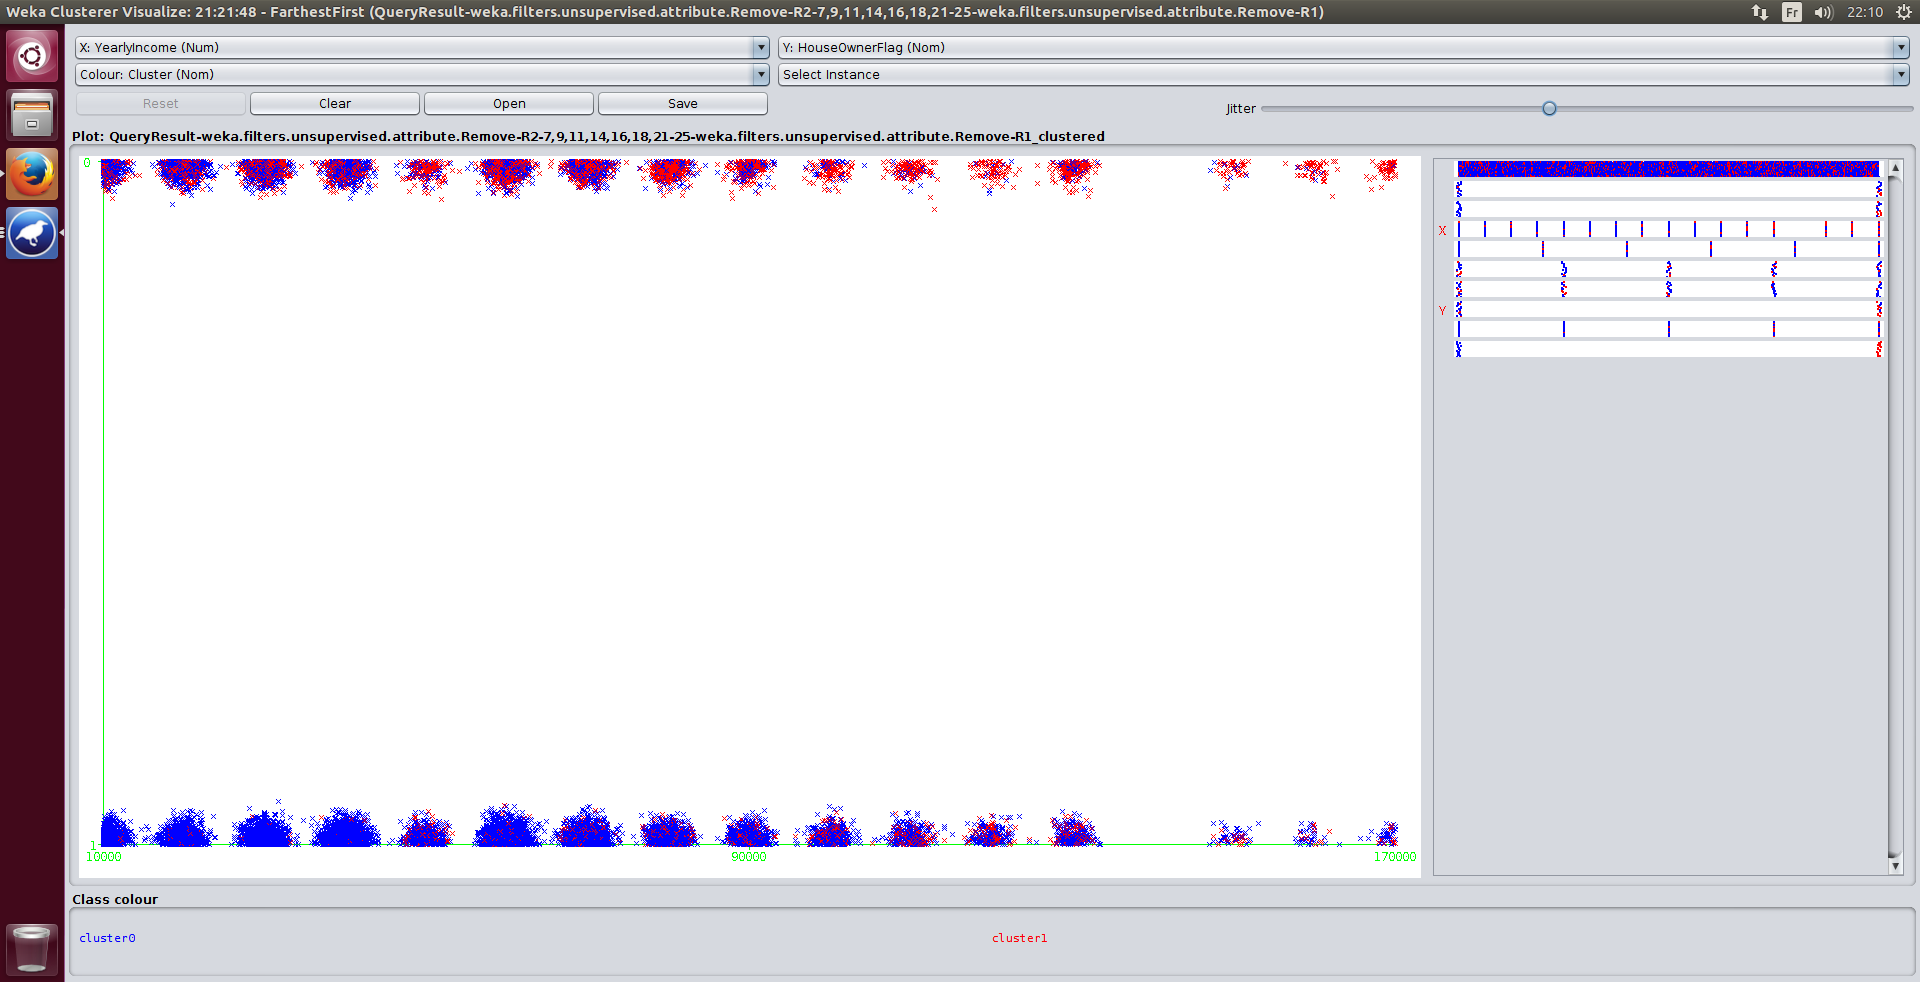
\includegraphics[width=1\linewidth, fbox]{img/clusterAvecJitter2.png}
    \caption{Clustering avec jitter et avec deux clusters}
    \label{sansJitter2}
\end{figure}


\subsection{8 clusters}

Pour cette génération (le jitter a été volontairement poussé pour permettre une meilleure visualisation des résultats), on constates que les revenus influencent certains clusters quand à l'état civil (marié ou non).
Il ne nous est pas en l'état possible de savoir pourquoi et de plus amples recherches seraient nécéssaires pour déterminer les facteurs communs de ces résultats.

\begin{figure}[H]
\centering
\begin{lstlisting}
=== Run information ===

Scheme:       weka.clusterers.FarthestFirst -N 8 -S 1
Relation:     QueryResult-weka.filters.unsupervised.attribute.Remove-R2-7,9,11,14,16,18,21-25-weka.filters.unsupervised.attribute.Remove-R1
Instances:    18484
Attributes:   8
              MaritalStatus
              Gender
              YearlyIncome
              TotalChildren
              EnglishEducation
              EnglishOccupation
              HouseOwnerFlag
              NumberCarsOwned
Test mode:    evaluate on training data


=== Clustering model (full training set) ===


FarthestFirst
==============

Cluster centroids:

Cluster 0
     M M 30000.0 0.0 Partial College Skilled Manual 0 1.0
Cluster 1
     S F 120000.0 5.0 Partial High School Professional 1 4.0
Cluster 2
     S F 160000.0 0.0 Graduate Degree Management 0 1.0
Cluster 3
     S M 10000.0 3.0 High School Manual 1 0.0
Cluster 4
     M M 170000.0 1.0 Bachelors Management 1 4.0
Cluster 5
     M F 30000.0 5.0 Graduate Degree Clerical 1 0.0
Cluster 6
     M F 120000.0 1.0 High School Professional 0 4.0
Cluster 7
     S M 130000.0 5.0 High School Management 0 4.0



Time taken to build model (full training data) : 0.07 seconds

=== Model and evaluation on training set ===

Clustered Instances

0       3967 ( 21%)
1       1534 (  8%)
2       1825 ( 10%)
3       3031 ( 16%)
4       2374 ( 13%)
5       3405 ( 18%)
6       1736 (  9%)
7        612 (  3%)
\end{lstlisting}
\caption{Output de l'éxécution avec 8 clusters}
\end{figure}

\begin{figure}[H]
    \centering
    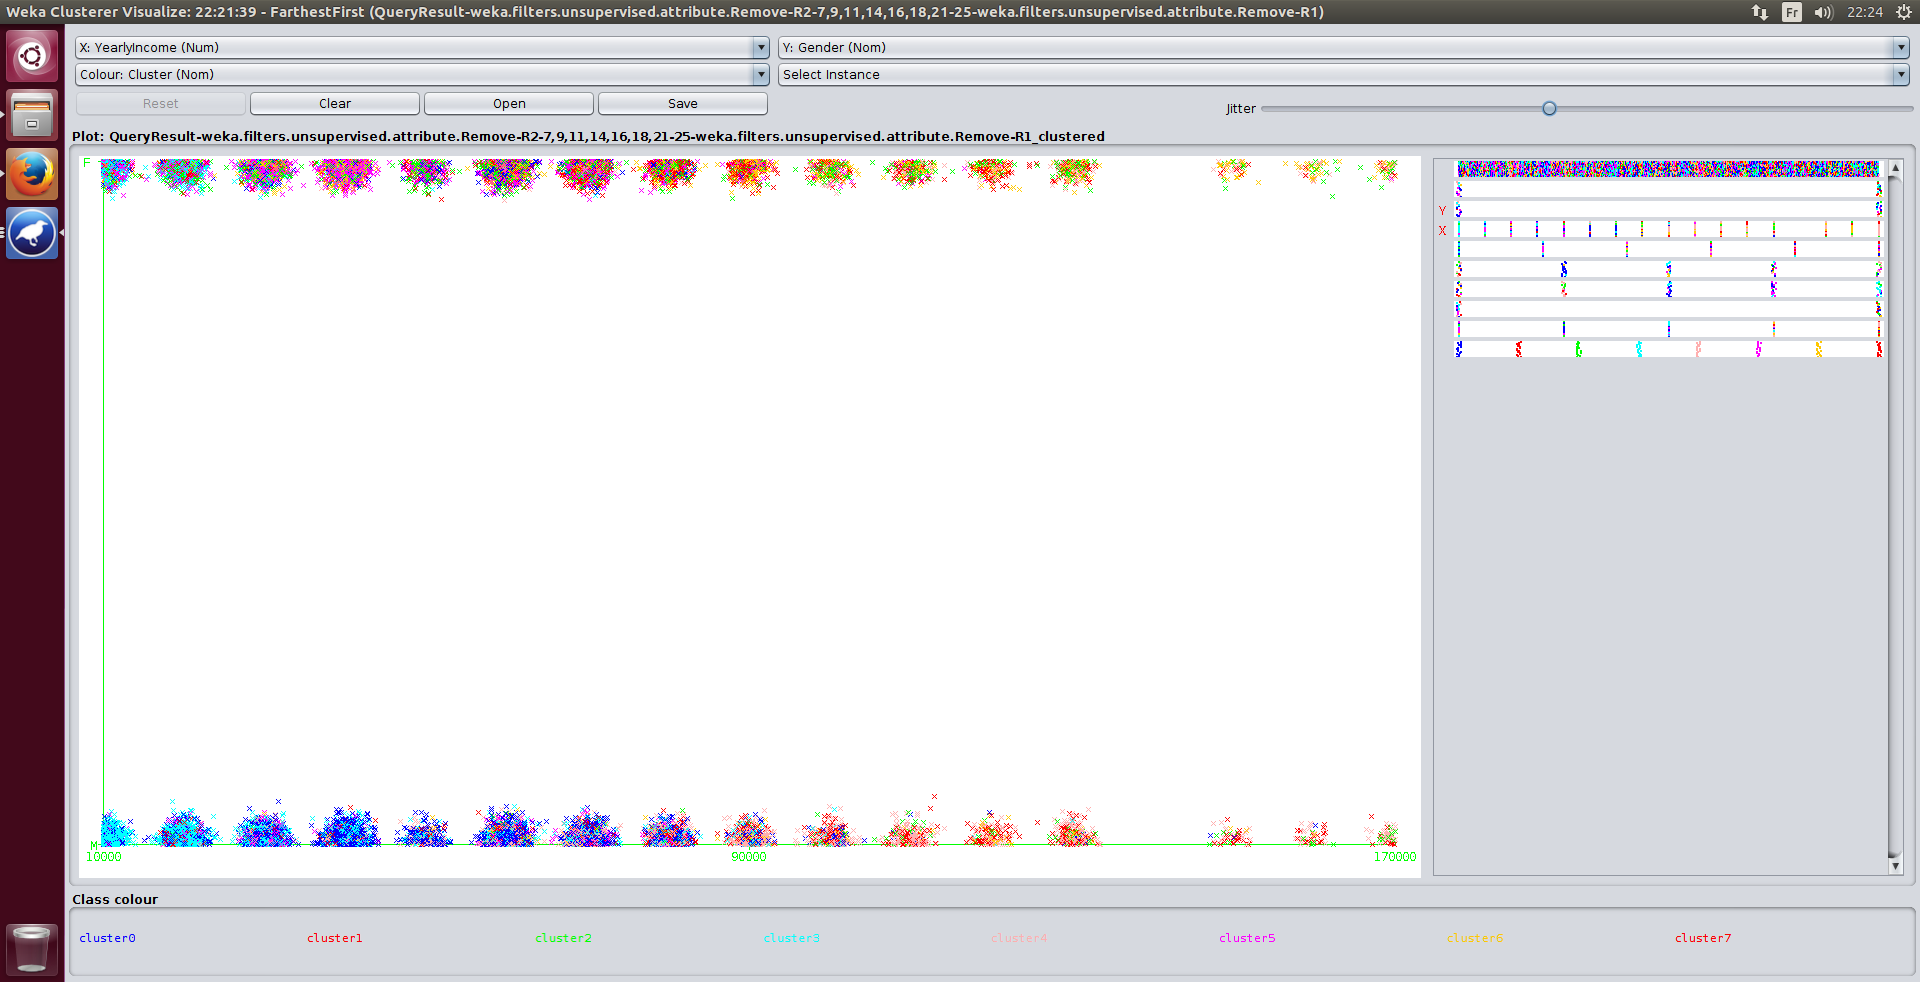
\includegraphics[width=1\linewidth, fbox]{img/clusterAvecJitter8.png}
    \caption{Clustering avec jitter et avec huit clusters}
    \label{sansJitter8}
\end{figure}
